\documentclass[10pt]{article}\usepackage[]{graphicx}\usepackage[]{color}
% maxwidth is the original width if it is less than linewidth
% otherwise use linewidth (to make sure the graphics do not exceed the margin)
\makeatletter
\def\maxwidth{ %
  \ifdim\Gin@nat@width>\linewidth
    \linewidth
  \else
    \Gin@nat@width
  \fi
}
\makeatother

\definecolor{fgcolor}{rgb}{0.345, 0.345, 0.345}
\newcommand{\hlnum}[1]{\textcolor[rgb]{0.686,0.059,0.569}{#1}}%
\newcommand{\hlstr}[1]{\textcolor[rgb]{0.192,0.494,0.8}{#1}}%
\newcommand{\hlcom}[1]{\textcolor[rgb]{0.678,0.584,0.686}{\textit{#1}}}%
\newcommand{\hlopt}[1]{\textcolor[rgb]{0,0,0}{#1}}%
\newcommand{\hlstd}[1]{\textcolor[rgb]{0.345,0.345,0.345}{#1}}%
\newcommand{\hlkwa}[1]{\textcolor[rgb]{0.161,0.373,0.58}{\textbf{#1}}}%
\newcommand{\hlkwb}[1]{\textcolor[rgb]{0.69,0.353,0.396}{#1}}%
\newcommand{\hlkwc}[1]{\textcolor[rgb]{0.333,0.667,0.333}{#1}}%
\newcommand{\hlkwd}[1]{\textcolor[rgb]{0.737,0.353,0.396}{\textbf{#1}}}%
\let\hlipl\hlkwb

\usepackage{framed}
\makeatletter
\newenvironment{kframe}{%
 \def\at@end@of@kframe{}%
 \ifinner\ifhmode%
  \def\at@end@of@kframe{\end{minipage}}%
  \begin{minipage}{\columnwidth}%
 \fi\fi%
 \def\FrameCommand##1{\hskip\@totalleftmargin \hskip-\fboxsep
 \colorbox{shadecolor}{##1}\hskip-\fboxsep
     % There is no \\@totalrightmargin, so:
     \hskip-\linewidth \hskip-\@totalleftmargin \hskip\columnwidth}%
 \MakeFramed {\advance\hsize-\width
   \@totalleftmargin\z@ \linewidth\hsize
   \@setminipage}}%
 {\par\unskip\endMakeFramed%
 \at@end@of@kframe}
\makeatother

\definecolor{shadecolor}{rgb}{.97, .97, .97}
\definecolor{messagecolor}{rgb}{0, 0, 0}
\definecolor{warningcolor}{rgb}{1, 0, 1}
\definecolor{errorcolor}{rgb}{1, 0, 0}
\newenvironment{knitrout}{}{} % an empty environment to be redefined in TeX

\usepackage{alltt}
\usepackage{amsmath}
\usepackage{amssymb}
\usepackage{geometry}
\usepackage{graphicx}
\usepackage{fullpage}
\usepackage{enumerate}
\IfFileExists{upquote.sty}{\usepackage{upquote}}{}
\begin{document}
\setlength\parindent{0pt}

Exam 3 Practice Problems\\
STAT 310, Spring 2021\\

\textbf{Exercise 1}.  The following scatterplot shows the association between price (in \$1,000's) and mileage (number of miles driven in 1,000's) for a sample of 30 used Honda Accords in 2017.  Also provided below is the output from fitting a simple linear regression model in R.\\

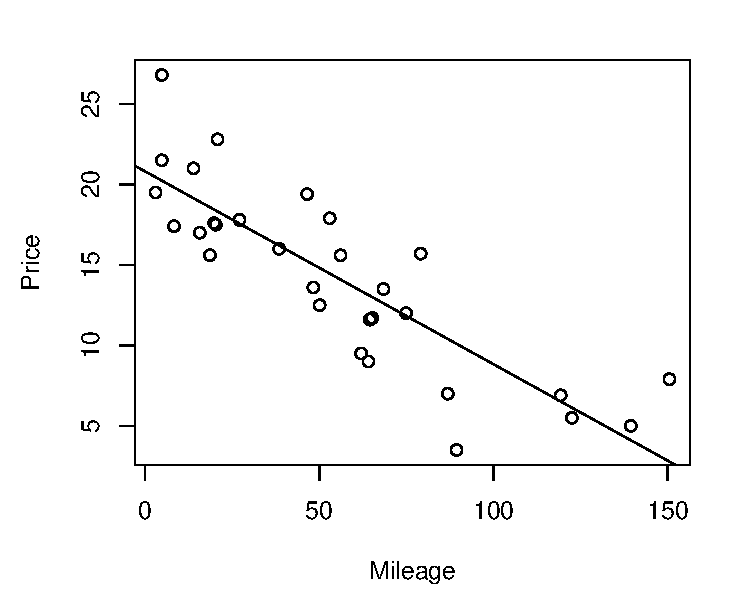
\includegraphics[scale=0.4]{figure/scatter_cars.pdf}

\begin{verbatim}
Coefficients:
            Estimate Std. Error t value Pr(>|t|)    
(Intercept)  20.8096     0.9529   21.84  < 2e-16 ***
Mileage      -0.1198     0.0141   -8.50 3.06e-09 ***
---
Signif. codes:  0 ‘***’ 0.001 ‘**’ 0.01 ‘*’ 0.05 ‘.’ 0.1 ‘ ’ 
\end{verbatim}

\medskip

\begin{enumerate}[(a)]
\item Do the data provide strong evidence of a linear association between the price of the used cars and the number of miles driven, i.e., is the slope of the regression line significantly different than 0? State the null and alternative hypothesis, report the test statistic and $p$-value, and state your conclusion. 
\vspace{3cm}
\item Calculate a 95\% confidence interval for the slope parameter $\beta_1$.
\vspace{4cm}
\item Do the results from the hypothesis test and confidence interval agree?  Explain.
\end{enumerate}

\newpage

% \textbf{Exercise 2}.  It is claimed that people get an average of 8 hours of sleep each night.  Suppose we want to conduct a hypothesis test to determine whether the average amount of sleep that CSUEB students get is significantly different than 8 hours.  Explain what is wrong with the following null and alternative hypothesis. \\
% 
% $H_0: \bar{x} = 8$\\
% $H_A: \bar{x} \neq 8$\\




\textbf{Exercise 2}.  A social worker at a local high school is interested in testing whether the average amount of sleep students get is significantly different than 8 hours, which is considered healthy. A random sample of $n=25$ students are interviewed.  The sample mean $\bar{x}=7.6$ and standard deviation $s=1.4$.  A boxplot of the data is also shown below.

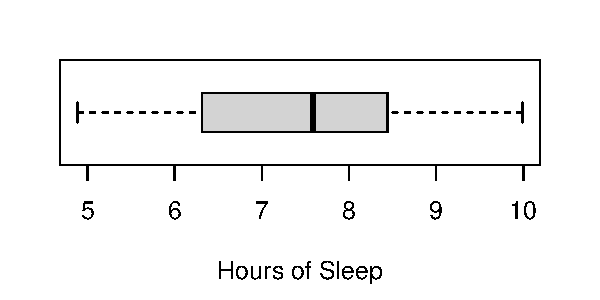
\includegraphics[scale = 0.6]{figure/boxplot_sleep.pdf}

\begin{enumerate}[(a)]
\item Which of the following is the correct null and alternative hypothesis for a two-sided test?
\begin{enumerate}[(i)]
\item $H_0: \bar{x} = 8$, $H_A: \bar{x} \neq 8$
\item $H_0: \mu = 8$, $H_A: \mu \neq 8$
\item $H_0: \bar{x} = 8.2$, $H_A: \bar{x} \neq 8.2$\\
\end{enumerate}

\item Check the conditions for the hypothesis test.
\vspace{3cm}

\item Calculate the test statistic.
\vspace{3cm}

\item Calculate the $p$-value and make a decision using $\alpha=0.05$.
\vspace{3cm}

\item What is the conclusion of the test in the context of the data?
\end{enumerate}

% \textbf{Exercise 3}.  In general, what are the conditions for performing a hypothesis test, or constructing a confidence interval, for one population mean $\mu$?


\end{document}
